%% <Schule/Chemie Protokoll/2-Chemie_Protokoll-2011-01-25.tex> Vorlageversion 1.2 <Robin Schneider>
\RequirePackage{RequirePackageRS}
%%% preamble (((
\documentclass[
  ngerman,
  % draft,
]{scrartcl}
%% Package list (((
\usepackage{
  defaultsRS,
  scrartclRS,
  timeRS,
  graphicRS,
  layoutRS,
  extensionsRS,
  docExtensionsRS,
  schoolRS,
  chemistryRS,
}
\usepackage[
  nohyperlinks,
  printonlyused,
]{acronym}
%% )))
%% Meta information (((
\usepackage[
  grumpy,
  dirty={* },
  % markifdirty,
]{gitinfo2}

\title{Chemie Praktikum}
\subject{Protokoll Nr.~1}
\author[*]{C. H.}
\author[*]{Jakob Schmusch}
\author[*]{Robin Schneider}
\SetCLASS{11}
%\SetURL{https://rsadmin.ath.cx/}
\SetGitURL{https://github.com/ypid/document-Chemie-Praktikum-K11}
\usepackage[
  type     = {CC},
  modifier = {by-nc-sa},
  version  = {3.0},
]{doclicense}
\SetCREATEDATE{2011}{01}{18}{13}{50}{23}
\SetABGABEDATUM{2}{2011}{02}{01}{1}
%% )))
\usepackage{
  footingChemMinutesRS,
  schoolPDFinfoRS,
  tableRS,
}
\hypersetup{pdfcreator={Robin Schneider}}
%% )))
\begin{document}
%%%%%%%%%%%
\section*{Aufgabe}
Herstellung von NaCl aus einer verunreinigten Lösung.

\vspace{0.1cm}
\begin{multicols}{2}
  \section*{Geräte}
  Bechergläser\\
  Trichter\\
  Filterpapier\\
  Filter mit Aktivkohle\\
  Reagenzgläser\\
  Reagenzglashalter\\
  Bunsenbrenner\\
  Spatel\\
  Holzspäne\\
  Sand\\
  Geranienöl

  % \columnbreak%

  \section*{Chemikalien}
  \includeListOfAbbreviationsChemistry%
\end{multicols}

\section*{Versuchsskizze}
\begin{center}
  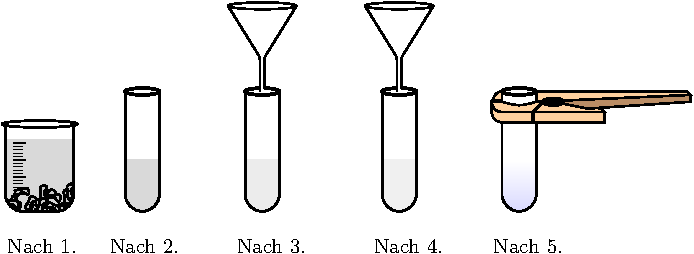
\includegraphics[scale=1.3]{pst-labo/Loesung_konzentrieren-pics.pdf}
\end{center}

\vspace{-0.2cm}
\section*{Durchführung}
%\begin{multicols}{2}
\begin{enumerate}
  \item Sedimentieren
  \item Dekantieren
  \item Filtrieren
  \item Adsorption
  \item Eindampfen
\end{enumerate}
%\end{multicols}

\section*{Beobachtungen}
\begin{enumerate}
  \item Die gröbsten Teile sind abgesunken.
  \item In dem dekantierten Becherglas blieb eine leicht gräuliche Flüssigkeit mit Schwebeteilchen zurück.
  \item Nachdem Filtrieren blieb eine klare Flüssigkeit ohne Schwebeteilchen.
  \item Nach der Adsorption roch die Flüssigkeit nicht mehr so stark.
  \item Das \ac{H2O} verdampfte und kondensierte teilweise am oberen kalten Rand des Reagenzglases wieder.
    Schließlich blieb weißes pulverförmiges \ac{NaCl}, das mit einem knisternden/knackenden Geräusch zersprang und so noch
feiner wurde.
\end{enumerate}

\section*{Auswertung}
\begin{enumerate}
  \item Das Sedimentieren und Dekantieren ist durch die unterschiedlichen Dichten $\rho $ der Stoffe möglich. Da
    dichtere Stoffe von der Gravitation stärker \enquote{angezogen} werden, sinken sie in Stoffen, die von selbst ausweichen
    (\zB{} Flüssigkeiten oder Gase) nach unten, wenn sie schwerer als der \enquote{Umgebungsstoff} (hier die Salzlösung) sind.
  \item Siehe 1.
  \item Bei der Filtration werden generell alle Partikel zurückgehalten,
    die größer als die Porengröße des Filters sind
    (hier wurden mit diesem mechanischen Trennverfahren die Schwebeteilchen zurückgehalten).
    Der Ölgehalt sinkt bei diesem Vorgang.
  \item Bei der wiederholten Filtration – dieses mal mit Einsatz von Aktivkohle – kam es zu einer Adsorption
    (Ablagerung von Flüssigkeiten und Gasen an der inneren Oberfläche fester Stoffe) an dem \ac*{6}.
  \item Das Eindampfen ist durch die unterschiedliche Siedetemperatur der Stoffe möglich.
\end{enumerate}

\appendix

\vfill
\printURLlong%
\doclicenseThis%
\printendsignature%
\end{document}
